\documentclass{beamer}

% !TEX root = slides.tex

\usetheme{Berlin}
\usecolortheme{beaver}

\AtBeginSection[]
{
  \begin{frame}
    \frametitle{Table of Contents}
    \tableofcontents[currentsection]
  \end{frame}
}

\definecolor{darkred}{rgb}{0.8,0,0}

\setbeamercolor{block title}{bg=darkred}
\setbeamercolor{section number projected}{bg=darkred}
\setbeamercolor{caption name}{fg=darkred}
\setbeamercolor{itemize item}{fg=darkred}
\setbeamercolor{itemize subitem}{fg=darkred}

\usepackage{amsmath,amsfonts,amssymb,amsthm}

\usepackage{booktabs}
\usepackage{graphicx}

\usepackage[justification=centering]{caption}

\usepackage{calc}

\setbeamercovered{transparent}

\newcommand{\troom}{\ensuremath{\hat{T}_{\mathrm{off}}}}
\newcommand{\hroom}{\ensuremath{\hat{h}_{\mathrm{off}}}}
\newcommand{\xa}{\ensuremath{\hat{x}_a}}

\newcommand{\irr}{\ensuremath{I}}
\newcommand{\irrnat}{\ensuremath{\hat{\irr}_{\mathrm{nat}}}}
\newcommand{\irrart}{\ensuremath{\irr_{\mathrm{art}}}}
\newcommand{\pho}{\ensuremath{A}}
\newcommand{\pow}{\ensuremath{P}}

\newcommand{\irrdelta}{\ensuremath{\irr_{\Delta}}}

\newcommand{\maxirrart}{\ensuremath{\irrart^{\max}}}
\newcommand{\maxpow}{\ensuremath{\pow^{\max}}}

\newcommand{\accirr}{\ensuremath{\irr_{\Sigma}}}
\newcommand{\accpho}{\ensuremath{\pho_{\Sigma}}}
\newcommand{\accpow}{\ensuremath{\pow_{\Sigma}}}

\newcommand{\optaccirr}{\ensuremath{\accirr^{\mathrm{opt}}}}
\newcommand{\maxaccpho}{\ensuremath{\accpho^{\max}}}
\newcommand{\minaccpho}{\ensuremath{\accpho^{\min}}}
\newcommand{\maxaccpow}{\ensuremath{\accpow^{\max}}}

\title{Identification and Control for Indoor Agriculture}
\author{Tom Neuh\"auser}
\date{\today}

\logo{
\includegraphics[width=1cm,keepaspectratio]{logos/tuLogoLongBlackWhite.pdf}}

\begin{document}

\frame{\titlepage}

\begin{frame}
    \frametitle{Table of Contents}
    \tableofcontents
\end{frame}

\begin{frame}
    \frametitle{Outline}
    
    \begin{figure}
        \centering
        \resizebox{!}{5.5cm}{
            \begin{tikzpicture}[node distance=1cm, font=\footnotesize]
                \node (datacollection) [section] {Data\\Collection};
                \node (plantphysiology) [section, right=of datacollection] {Plant\\Physiology};
                \node (neuralnetwork) [section, right=of plantphysiology] {Neural\\Network};

                \node (costfunction) [section, below=of datacollection, xshift=1.5cm, yshift=-0.5cm] {Cost\\Function};
                \node (constraints) [section, right=of costfunction] {Constraints};

                \node (identification) [chapter, label=above:Identification, fit=(datacollection) (plantphysiology) (neuralnetwork)] {};
                \node (control) [chapter, label=above:Control, fit=(costfunction) (constraints)] {};
                \node (casestudy) [chapter, below=of control] {Case Study};

                \draw [arrow] (datacollection) -- (plantphysiology);
                \draw [arrow] (plantphysiology) -- (neuralnetwork);

                \draw [arrow] (identification.east) -| +(0.5,-1) -- +(-9.5,-1) |- (control.west);
                \draw [arrow] (costfunction) -- (constraints);
                \draw [arrow] (control.east) -| +(0.5,-1) -- +(-9.5,-1) |- (casestudy.west);
            \end{tikzpicture}
        }
    \end{figure}
\end{frame}

% !TEX root = slides.tex

\section{Introduction}

\begin{frame}
    \frametitle{Sample frame title}
    \begin{block}{Block}
        This is some text in the first frame. This is some text in the first frame. This is some text in the first frame.
    \end{block}
\end{frame}
% !TEX root = slides.tex

\section{Identification}

\begin{frame}
    \frametitle{Sample frame title}
    This is some text in the first frame. This is some text in the first frame. This is some text in the first frame.
\end{frame}
% !TEX root = slides.tex

\section{Control}

\newcommand*{\WidestLeftHandSide}{\small$\accpho(j+1 \mid k)$}
\newcommand*{\WidestRightHandSide}{\small$\mathcal{N}\left(\left[\irr(j \mid k), \, \troom(j \mid k), \, \hroom(j \mid k), \, \xa(j \mid k)\right]^T\right),$}

\begin{frame}<1>[label=mpc1]
    \frametitle{Model Predictive Control Problem I}
    Solve the optimization problem
    {\footnotesize
        \begin{equation*}
            \min_M \, \sum_{j=k}^{K-1} \left\vert \irr(j \mid k) - \irr(j-1 \mid k) \right\vert + V\left(\left[\accirr(K \mid k), \, \accpho(K \mid k), \, \accpow(K \mid k)\right]^T\right)
        \end{equation*}
    }

    \onslide<6->{
        subject to
    }
    {\small
        \begin{align*}
            \onslide<6->{
                \makebox[\widthof{\WidestLeftHandSide}][r]{$\accirr(j+1 \mid k)$} &= \makebox[\widthof{\WidestRightHandSide}][l]{$\accirr(j \mid k) + \tau \cdot \frac{1}{\mathrm{C}_{\irr}} \cdot \irr(j \mid k),$} \\
                \accpho(j+1 \mid k) &= \accpho(j \mid k) + \tau \cdot \frac{1}{\mathrm{C}_{\pho}} \cdot \pho(j \mid k), \\
                \accpow(j+1 \mid k) &= \accpow(j \mid k) + \tau \cdot \frac{1}{\mathrm{C}_{\pow}} \cdot \pow(j \mid k), \\
            }
        \end{align*}
    }
\end{frame}

\begin{frame}<2-4>
    \frametitle{Terminal Cost Function}
    The terminal cost function equals the weighted sum of
    
    \begin{align*}
        &V_{\irr}\left(\accirr(K \mid k)\right) = 
        \begin{cases}
            \optaccirr - \accirr(K \mid k) & \text{if } \accirr(K \mid k) \leq \optaccirr \\
            0 & \text{else}
        \end{cases} \\[0.5cm]
        \onslide<3->{
            &V_{\pho}\left(\accpho(K \mid k)\right) = - \accpho(K \mid k)\\[0.5cm]
        }
        \onslide<4>{
            &V_{\pow}\left(\accpow(K \mid k)\right) = \accpow(K \mid k)
        }
    \end{align*}

\end{frame}

\againframe<5-6>{mpc1}

\begin{frame}<6-7>[label=mpc2]
    \frametitle{Model Predictive Control Problem II}
    {\small
        \begin{align*}
            \onslide<6->{
                \makebox[\widthof{\WidestLeftHandSide}][r]{$\irr(j \mid k)$} &= \makebox[\widthof{\WidestRightHandSide}][l]{$\irrnat(j \mid k) + \irrart(j \mid k),$} \\
            }
            \onslide<7->{
                \pho(j \mid k) &= \mathcal{N}\left(\left[\irr(j \mid k), \, \troom(j \mid k), \, \hroom(j \mid k), \, \xa(j \mid k)\right]^T\right), \\
            }
            \onslide<11->{
                \pow(j \mid k) &= \frac{\maxpow}{\maxirrart} \cdot \irrart(j \mid k), \\
            }
            \onslide<12->{
                \irrart(j \mid k) &\geq 0, \\
                \irrart(j \mid k) &\leq \maxirrart, \\
            }
            \onslide<13->{\accpow(K \mid k) &\leq \maxaccpow}
        \end{align*}
    }

    \onslide<14>{
        for $j = k , \ldots , K-1$ as well as with $\accirr(k \mid k) = \accirr(k)$, $\accpho(k \mid k) = \accpho(k)$ and $\accpow(k \mid k) = \accpow(k)$.
    }
\end{frame}

\begin{frame}<8>
    \frametitle{Neural Network Formulation I}

    A three-layer neural network can be represented by constructing mixed-integer programming formulations for its units.

    \vspace{0.5cm}

    \begin{figure}
        \centering
        \resizebox{8cm}{!}{
            \begin{tikzpicture}[node distance=1em and 2em, >=latex, font=\footnotesize]
                \node[data] (x1) {$x_1$};
                \node[data, below=of x1] (x2) {$x_2$};
                \node[circle, below=of x2] (dots) {\rotatebox{90}{$\cdots$}};
                \node[data, below=of dots] (xn) {$x_n$};

                \node (helper) at ($(x2)!0.5!(dots)$) {};

                \node[operation, right=of helper, xshift=2em] (sum) {$\sum_{i=1}^n w_i \cdot x_i + b$};
                \node[data, right=of sum] (y) {$y$};
                \node[operation, right=of y] (max) {$\max\{0,y\}$};
                \node[data, right=of max] (z) {$z$};

                \node[above=of sum, yshift=1em] (b) {$b$};  

                \draw [->] (x1) -- node[near start, above=0.25em] {$w_1$} ($(sum.west) + (0,0.2)$);
                \draw [->] (x2) -- node[near start, above] {$w_2$} (sum.west);
                \draw [->] (xn) -- node[near start, above=0.25em] {$w_n$} ($(sum.west) - (0,0.2)$);

                \draw [->] (b) -- (sum);

                \draw [->] (sum) -- (y);

                \draw [->] (y) -- (max);

                \draw [->] (max) -- (z);
            \end{tikzpicture}
        }
        \caption{Rectified linear unit.}
    \end{figure}
\end{frame}

\begin{frame}<9>
    \frametitle{Neural Network Formulation II}
    
    A mixed-integer programming formulation for a rectified linear unit can be constructed as 
    {\small
    \begin{align*}
        z &\geq 0, \\
        z &\geq \left(\sum_{i=1}^n w_i \cdot x_i + b\right), \\
        z &\leq \left(\sum_{i=1}^n w_i \cdot x_i + b\right) - M^- \cdot (1-\delta), \\
        z &\leq M^+ \cdot \delta
    \end{align*}
    }

    where $\delta \in \{0, \, 1\}$ is a binary variable and $M^-, M^+ \in \mathbb{R}$ are constants.

\end{frame}

\againframe<10->{mpc2}
% !TEX root = slides.tex

\section{Case Study}

\againframe{overview}

\begin{frame}
    \frametitle{Simulation}
    
    \begin{itemize}
        \onslide<1->{
            \item Model predictive control
            \begin{itemize}
                \item Formulated using Pyomo and OMLT
                \item Solved using CBC 
            \end{itemize}
        }
        \onslide<2->{
            \item Manual control
            \begin{itemize}
                \item 16 hours photoperiod starting at 4 o'clock
                \item $12.9 \, \mathrm{mol} \, \mathrm{m}^{-2} \, \mathrm{d}^{-1}$ optimal accumulated irradiance
                \item $3.8 \, \mathrm{mol} \, \mathrm{m}^{-2} \, \mathrm{d}^{-1}$ average accumulated natural irradiance 
            \end{itemize}
        }
        \onslide<3>{
            \item Forecasts of the uncertain inputs
            \begin{itemize}
                \item Solar forecasts from external service
                \item Persistence forecast of temperature and humidity
                \item Seasonal persistence forecast of carbon dioxide concentration 
            \end{itemize}
        }
    \end{itemize}
\end{frame}

\begin{frame}
    \frametitle{Results}
    \begin{figure}
        \centering
        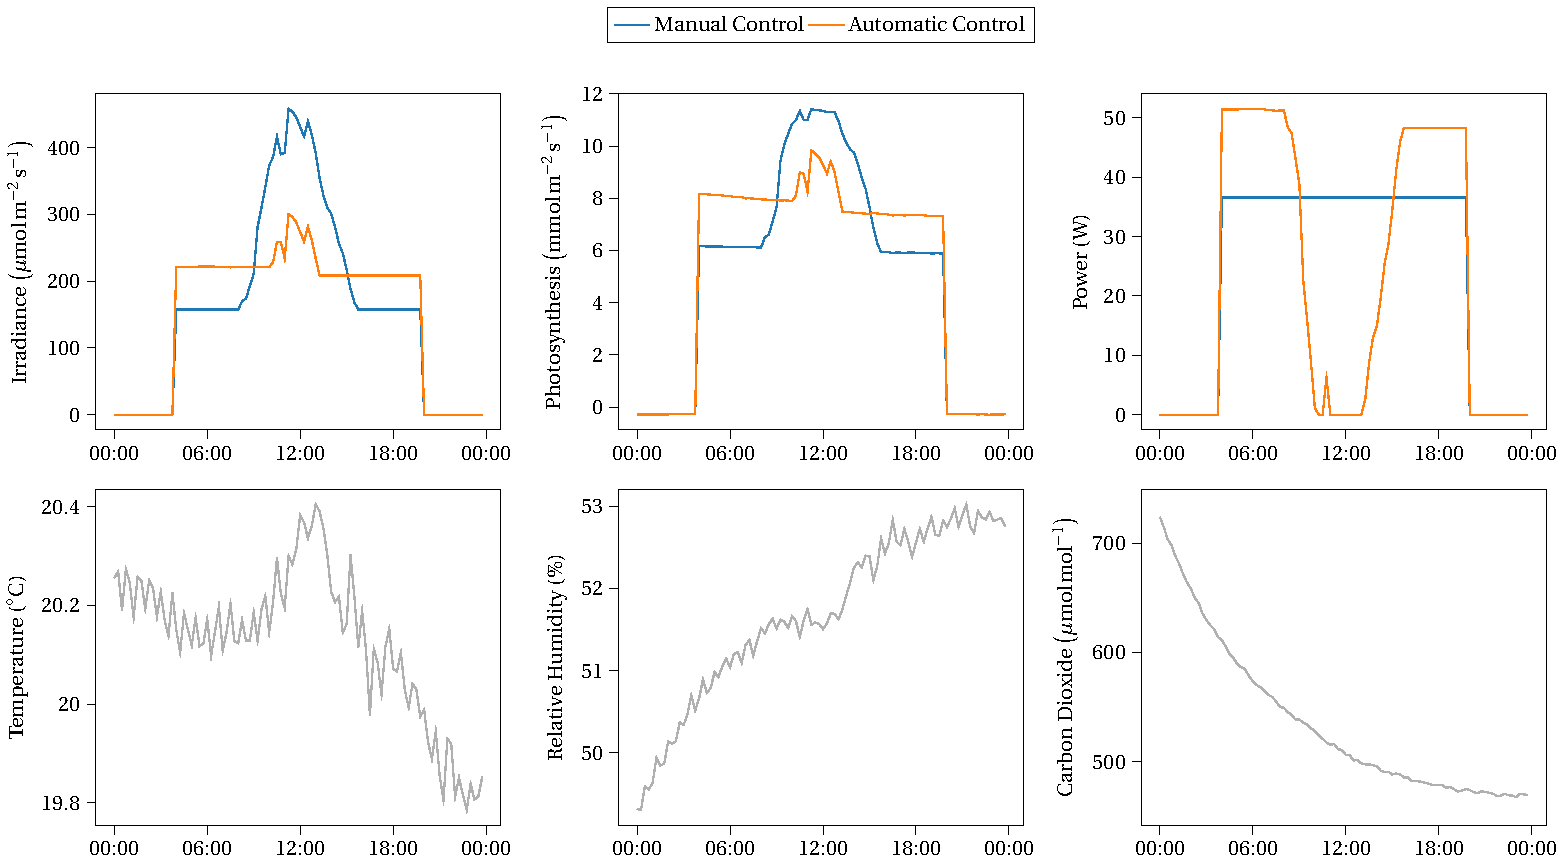
\includegraphics[scale=0.3]{figures/casestudy.pdf}
        \caption{Results of the simulation case study for 10th December 2022.}
    \end{figure}
\end{frame}

\begin{frame}
    \frametitle{Results}
    \begin{table}
        \centering
        \resizebox{10cm}{!}{
            \begin{tabular}{lrrrrr}
            \toprule
            & 10.12.2022 & 11.12.2022 & 12.12.2022 & 13.12.2022 & 14.12.2022 \\
            \midrule
            manual & 13.59 & 11.71 & 10.38 & 14.86 & 14.6 \\
            automatic & 12.9 & 11.79 & 10.45 & 12.95 & 12.9 \\
            \bottomrule
            \end{tabular}
        }
        \caption{Accumulated irradiances $\left(\mathrm{mol} \, \mathrm{m}^{-2} \, \mathrm{d}^{-1}\right)$}
    \end{table}
\end{frame}

\begin{frame}
    \frametitle{Results}
    \begin{table}
        \centering
        \resizebox{10cm}{!}{
            \begin{tabular}{lrrrrr}
            \toprule
            & 10.12.2022 & 11.12.2022 & 12.12.2022 & 13.12.2022 & 14.12.2022 \\
            \midrule
            manual & 742.81 & 659.95 & 658.19 & 854.64 & 784.81 \\
            automatic & 832.15 & 674.58 & 670.92 & 1065.63 & 933.17 \\
            \bottomrule
            \end{tabular}
        }
        \caption{Ratios of accumulated photosynthetic rates per power unit $\left(\mathrm{mmol} \, \mathrm{m}^{-2} \, \mathrm{d}^{-1} \; \slash \; \mathrm{kWh}\right)$}
    \end{table}
\end{frame}
% !TEX root = slides.tex

\section{Conclusion}

\begin{frame}
    \frametitle{Conclusion}
    \begin{center}
        {\Large
            \textit{We can grow more with less.}
        }
    \end{center}
\end{frame}

\end{document}